\documentclass[12pt, a4paper]{article}

\usepackage{polski}
\usepackage[utf8]{inputenc}

\usepackage[dvipsnames]{xcolor}
\usepackage[hyphens]{url}
\usepackage{graphicx}

\title{Hałaseon}

\date{\today}


\begin{document}

\begin{titlepage}
	\begin{flushright}
	{\large \color{Goldenrod} \emph{\textbf{Muzyka z radiowęzła to szum.}} \linebreak}
	~prezes Ryszard Szubartowski
	\end{flushright}
	\centering
	\vspace{1.5 cm}
	{\scshape Projekt na konkurs Akademia Kodowania\par}
	\vspace{1.5 cm}
	{\huge\bfseries Hałaseon\par}
	\vspace{0.1cm}
	{\scshape\Large czyli pomiar hałasu dla dobra uczniów\par}
	\vspace{2cm}
	{\Large\itshape Przemysław Buczkowski\linebreak Paweł Wieczorek\par}
	\vfill
	pod opieką\par
	mgr. inż. \textsc{Konrada Buzaka}

	\vfill

	{\large \today\par}
\end{titlepage}

\tableofcontents

\vfill \pagebreak

\section{Wstęp}

Hałas jest jednym z~cywilizacyjnych zagrożeń czyhających na nasze zdrowie. Tak jak fast foody powodują cukrzycę~i~otyłość, a~wielogodzinne przesiadywanie przed komputerem wady postawy, tak przebywanie w miejscach o~podwyższonym natężeniu hałasu powoduje, że słyszymy znacznie gorzej niż ludzie żyjący jeszcze kilkadziesiąt lat temu.

Jakie są to miejsca? Nam w pierwszej kolejności przychodzi do głowy nasze liceum w trakcie przerwy. Setki uczniów upchanych na wąskim korytarzu i hip-hopowa muzyka z radiowęzła. Jeżeli ktoś nie lubi chodzić na koncerty muzyczne, to ciężko sobie wyobrazić, by miał gdzieś do czynienia z większym poziomem hałasu.

W szkołach województwa śląskiego przeprowadzono pomiary, z których wynikło, że średni poziom hałasu to 85 decybeli\cite{dz}, podczas gdy poziom bezpieczny to 70 decybeli\cite{wikihalas}. Trzeba tu wspomnieć, że decybel jest jednostką logarytmiczną, więc dźwięk o natężeniu około 6 decybeli większym jest odbierany przez człowieka jako dwukrotnie głośniejszy.

Nie potrzeba skomplikowanych badań, żeby poznać tego skutki. Wielu uczniów jak i nauczycieli skarży się na bóle głowy i uszu, migreny, nie jest w stanie się skupić i odczuwa zmęczenie przez codzienne przebywanie w tak głośnym środowisku. W dalszej części scenariusza zawarliśmy krótki przegląd wiedzy naukowej na ten temat.

Celem naszego przedsięwzięcia jest zbudowanie urządzenia, dzięki któremu będzie można skutecznie mierzyć poziom hałasu w różnych miejscach budynku szkoły. Projekt takiej sondy jest przedstawiony w niniejszym dokumencie. Po jej zbudowaniu wypróbujemy je w naszej szkole i określimy skalę problemu dla niej. Zawarliśmy też tutaj rozmaite nasze propozycje, jak wykorzystać dane, które będą zbierane przez urządzenie i~w~efekcie pomóc w~redukcji hałasu w~środowisku szkolnym i nie tylko.

\section{Szkodliwość hałasu w pigułce}
Z hałasem spotykamy się na co dzień -- w pracy, na ulicy, czasem w domu. Jednak rzadko zdajemy sobie sprawę, jak niekorzystnie wpływa on na nasze zdrowie i lekceważymy jego skutki. Od zaledwie 70 dB pojawiają się niekorzystne zmiany w organizmie -- nadciśnienie, zaburzenie pracy żołądka czy problemy psychiczne\cite{70db}. W badaniach przeprowadzonych w ciągu kilku ostatnich lat stwierdzono, że hałas ma zły wpływ na ciążę i prowadzi do zaburzeń w rozwoju kości noworodka (głównie zębów). Ponadto skutkuje występowaniem wrzodów żołądka oraz przyspiesza proces starzenia się.

Powyżej 90 dB dochodzi do ubytków słuchu. Są to zmiany nieodwracalne, których skutki łagodzi się poprzez stosowanie aparatów słuchowych. Po przekroczeniu 120 dB istnieje niebezpieczeństwo mechanicznego uszkodzenia słuchu, które prowadzi do trwałej głuchoty.

Obecnie problem hałasu przestaje być lekceważony, czego dowodem są działania podejmowane przez instytucje ustawodawcze państw, które to wprowadziły jasno określone granice, po przekroczeniu których uznaje się dane zajęcie za głośne i nakłada się obowiązek noszenia elementów chroniących słuch. W niektórych szkołach zastąpiono głośne dzwonki lekcyjne komunikatami z głośników oraz zaczęto edukować uczniów w zakresie spokojniejszego spędzania przerw.

\section{Zbierane dane i ich zastosowania}

Głównym zadaniem urządzenia jest zbieranie oraz prezentowanie w przyjemnej formie wizualnej danych określających poziom hałasu w różnych miejscach szkoły. Zastosowanie więcej niż jednej sondy pozwala na łatwe objęcie pomiarem całego terenu placówki edukacyjnej, a także umożliwia uzyskanie bardziej wiarygodnych danych. Dzięki umieszczeniu precyzyjnego (w stosunku do funkcji jaką ma pełnić) czujnika poziomu natężenia dźwięku dane zebrane przez system umożliwią wyciągnięcie cennych wniosków.

\subsection{Procedura pomiarowa}

Dane pobierane będą co sekundę w cyklach 5 sekundowych. Z każdej partii danych usuwane będą dwie skrajne wartości, a z reszty liczona średnia logarytmiczna według poniższego wzoru\cite{log}:

\Large
\begin{equation}
L_{sr} = 10*\log_{10}\left[\frac{1}{n}\displaystyle\sum_{i=1}^{n}10^{\frac{L_i}{10}}\right]
\end{equation}
\normalsize

Gotowe dane będą zapisywane w bazie danych na sondzie.

\subsection{Proponowane zastosowania}

Możliwości urządzenia ogranicza tylko nasza wyobraźnia. Może zostać wykorzystane do zbierania informacji statystycznych pozwalających opracowywać program dydaktyczny zwiększający/zmniejszający nacisk na kwestie zachowania się na przerwach. W połączeniu z badaniami (np. ankietami) może służyć do pomiaru wpływu hałasu na komfort i zdrowie uczniów.

Co więcej, z pomocą uzyskanych informacji można dostosowywać głośność dzwonków szkolnych do panujących aktualnie warunków akustycznych -- byłaby ona zmniejszana w przypadku stwierdzenia ciszy w danym miejscu.

Poza tym istnieje możliwość wprowadzania poprawek do planu lekcji prowadzących do równomiernego rozłożenia hałasu na cały budynek szkolny. Dzięki zastosowaniu interfejsów Bluetooth oraz Wi-Fi, w które wyposażona jest platforma Intel Edison, możliwa jest łatwa rozbudowa systemu poprzez dokupienie większej ilości urządzeń i podłączenie ich do jednej sieci.

Wspomniane wyżej interfejsy bezprzewodowe pozwalają ograniczyć ilość wymaganego okablowania do minimum: niezbędne jest jedynie zasilanie, które może być realizowane z wykorzystaniem baterii bądź akumulatora litowo-jonowego.

W rezultacie zmniejszenie hałasu oraz głośności dzwonków uprzyjemni życie uczniom i mieszkańcom budynków znajdujących się w pobliżu placówki oświatowej.

\section{Budowa sondy}

Elementy wykorzystane w projekcie:
\begin{itemize}
\item płytka Intel Edison wraz modułem rozszerzeń Arduino Breakout Board,
\item Grove Base Shield V2,
\item mikrofon,
\item wyświetlacz 16x2 z podświetleniem RGB,
\item przycisk „Grove Button”
\item potencjometr,
\item zasilacz 9V.
\end{itemize}

Sercem całego urządzenia będzie platforma Intel Edison wraz z modułem Grove Base Shield V2. Do niego zostanie podłączony wyświetlacz LCD 16x2 (poprzez interfejs I2C), mikrofon oraz reszta wymienionych elementów. Łącznie wykorzystane zostaną 2 złącza analogowe, 1 cyfrowe i 1~magistrala I2C. 

Do obsługi sondy zastosowane zostaną przycisk oraz potencjometr, służący do regulowania czułości. Oprócz tego podczas przerw, bądź po naciśnięciu przycisku, będzie zapalać się podświetlenie wyświetlacza celem zobrazowania aktualnego poziomu hałasu (czym bardziej czerwony, tym jest głośniej).

Urządzenie będzie zasilanie napięciem DC 9V z zewnętrznego zasilacza. Opcjonalnie ma istnieć możliwość podłączenia do niego akumulatora lub baterii (do zasilania, bądź zapewnienia jego awaryjnego podtrzymania).

Sondy będą komunikować się ze sobą z wykorzystaniem sieci lokalnej, do której zostaną podłączone z wykorzystaniem Wi-Fi, bądź na krótkie odległości -- poprzez Bluetooth. Ponadto urządzenie będzie dysponować zewnętrznym portem USB, który umożliwi podłączenie go do komputera.

Przy wykorzystaniu wyżej wymienionego portu USB możliwa będzie wstępna konfiguracja urządzenia -- nazwa sieci, hasło, adres IP, itp. -- oraz aktualizacja oprogramowania. Dzięki tym funkcjom sonda będzie mogła otrzymywać na bieżąco nowe funkcjonalności oraz poprawki błędów. Ponadto uprości to znacząco nastawianie urządzenia, gdyż wykorzystany zostanie do tego przejrzysty kreator.

\section{Oprogramowanie sondy}

Projektowane urządzenie działa pod kontrolą systemu Yocto Linux. Instalacja systemu będzie się odbywała poprzez podłączenie sondy do komputera PC, na którym zainstalowany jest zaprojektowany przez nas instalator, przez który będzie można skonfigurować podstawowe funkcje urządzenia.

Dane przechowywane są w bazie SQLite zarządzanej przez framework Django. W oparciu o ten framework wykonaliśmy interfejs prezentujący zebrane dane. Wpisaliśmy w niego przykładowe dane i uruchomiliśmy na naszym serwerze.

\textbf{Działający projekt interfejsu:} \url{https://halaseon.1mi.pl}

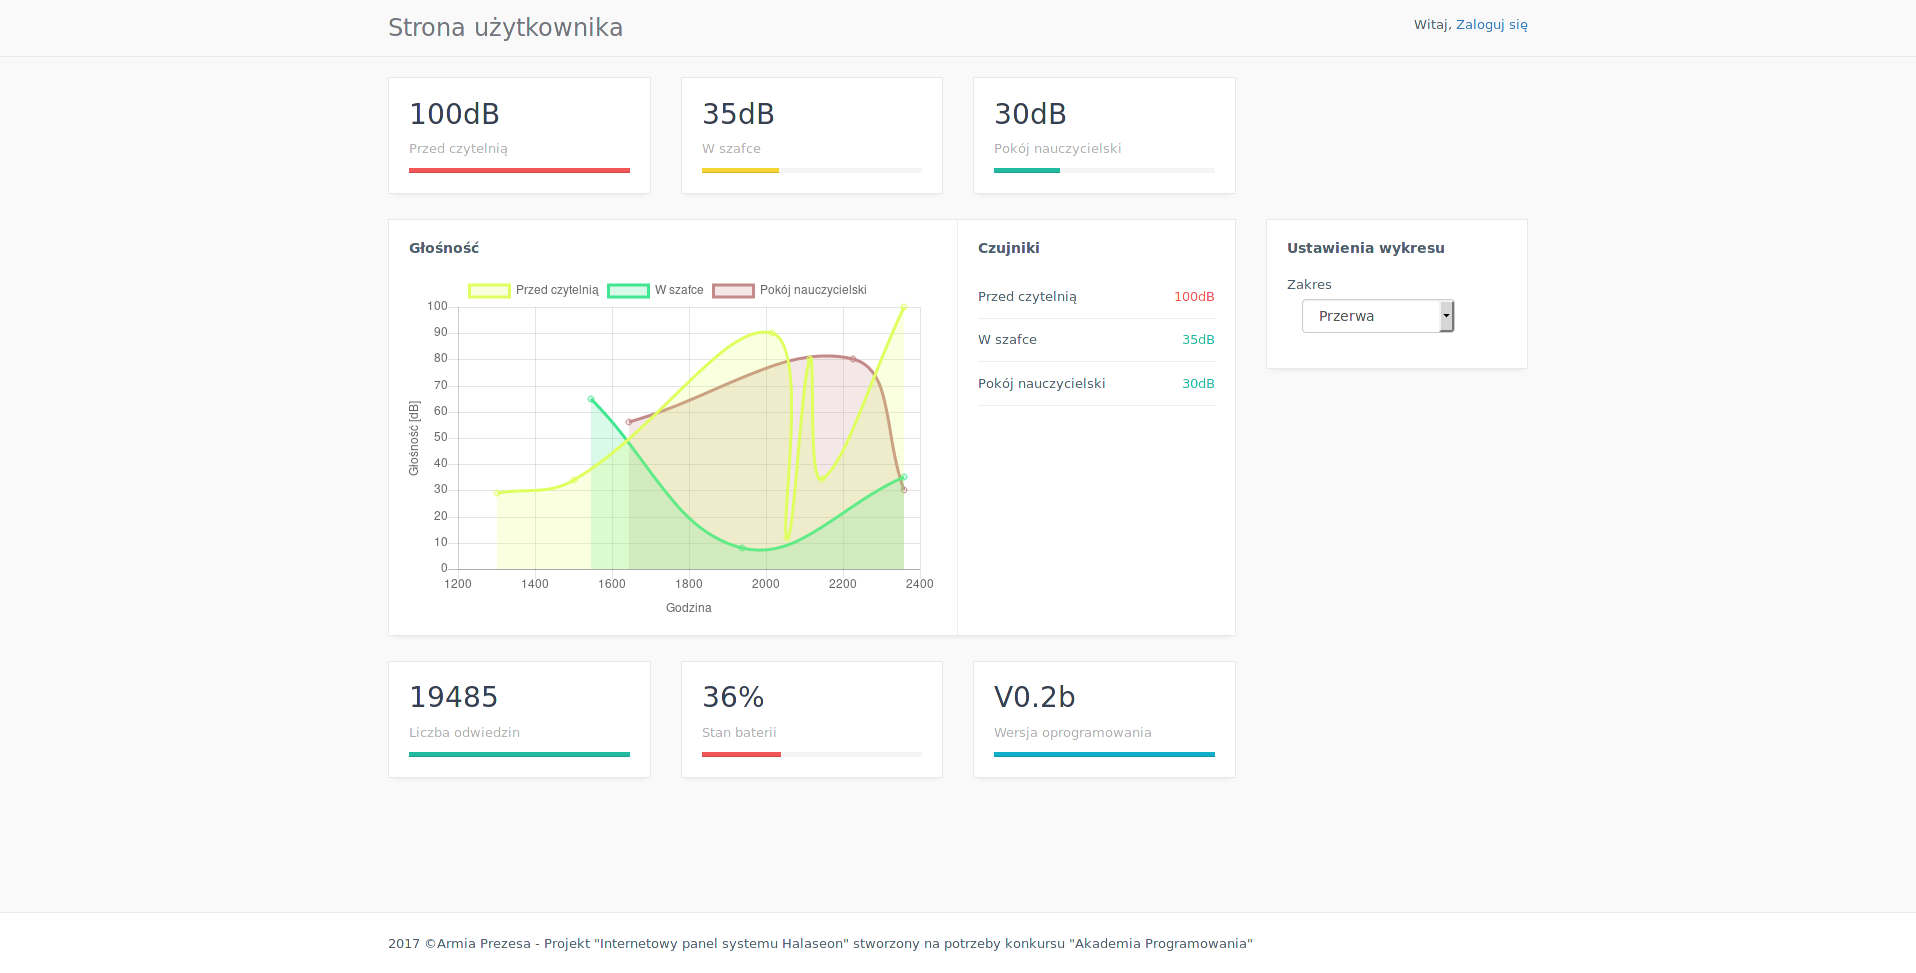
\includegraphics[width=\textwidth]{web_page1.png}
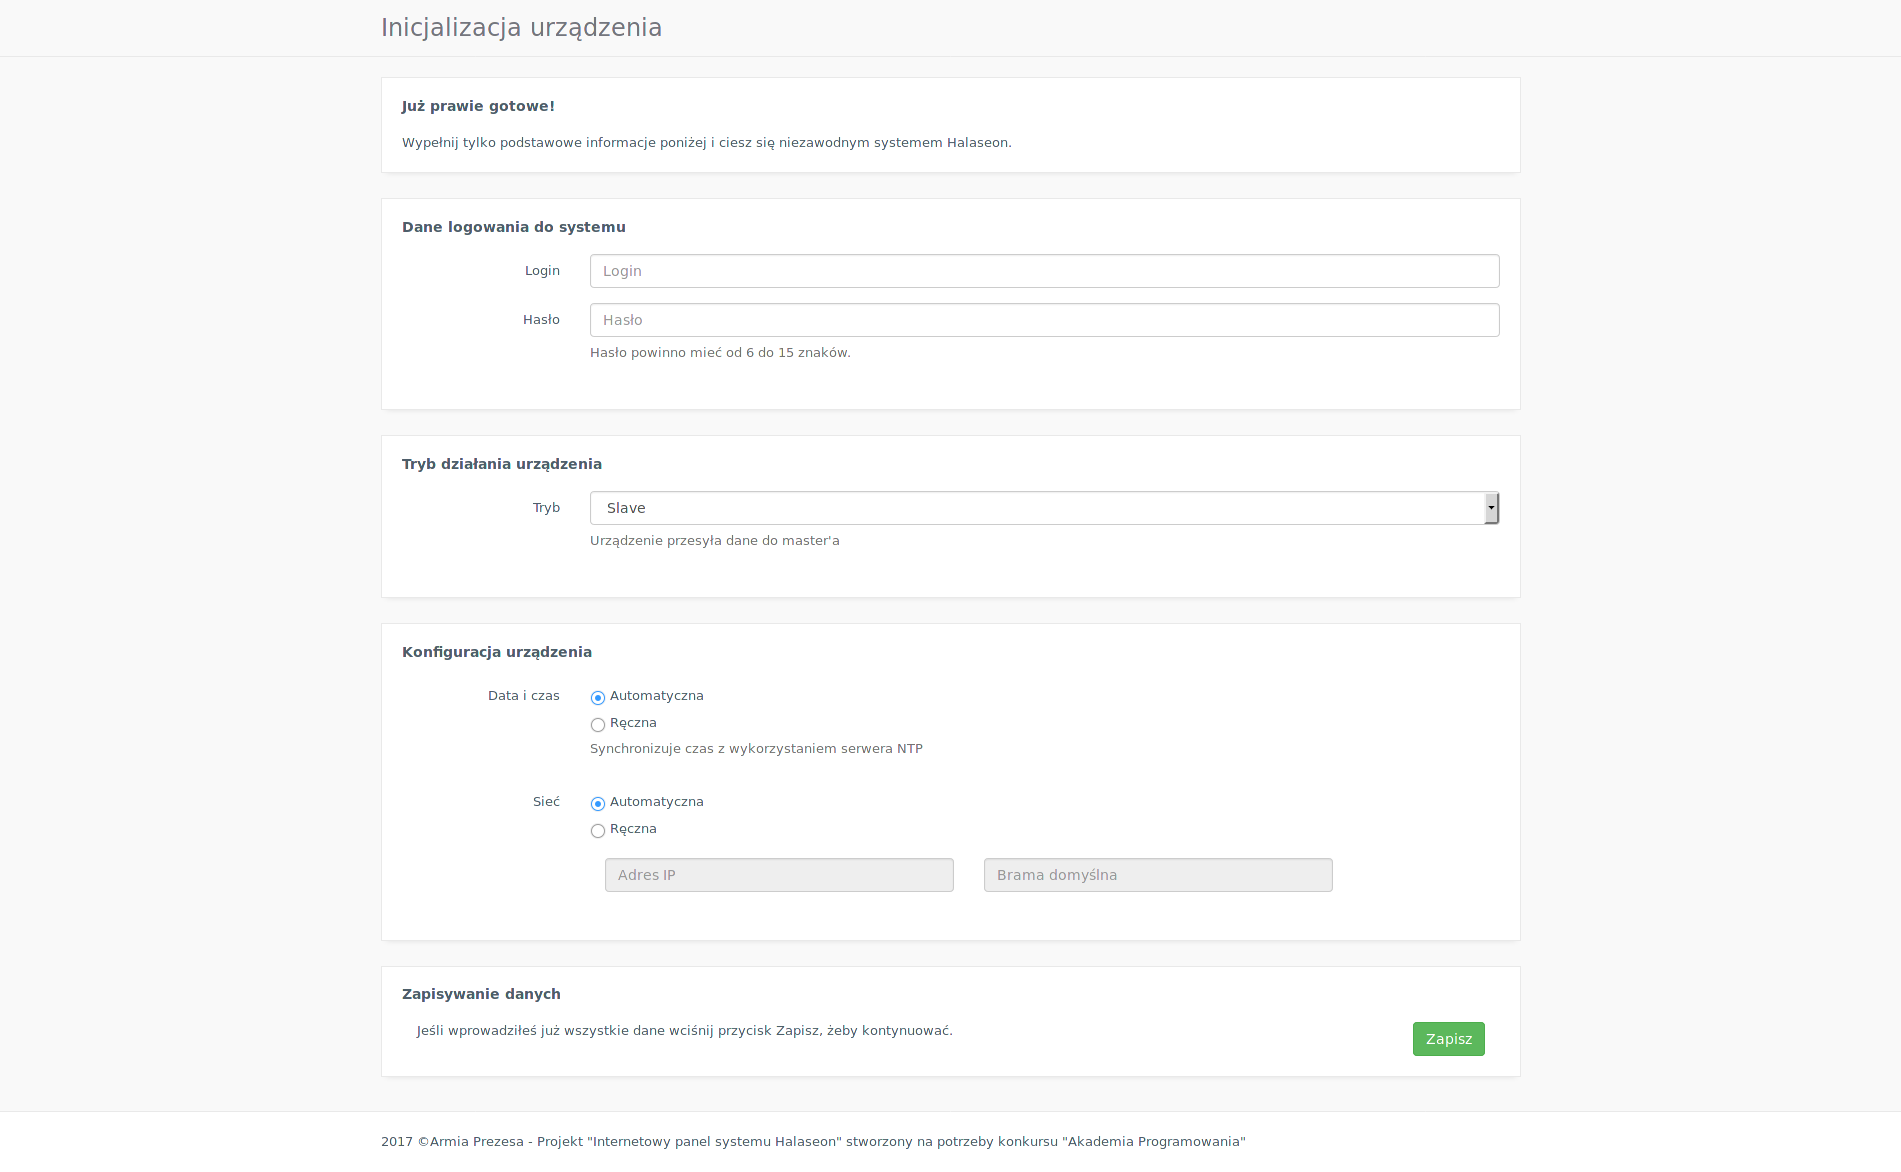
\includegraphics[width=\textwidth]{web_page2.png}

Zbieranie danych odbywać się będzie z użyciem napisanego przez nas skryptu w języku Python 3, przy wykorzystaniu bibliotek udostępnianych przez producenta elementów. 

Dzięki zastosowanemu oprogramowaniu, będziemy mogli położyć odpowiedni nacisk na kwestie bezpieczeństwa. Nikt przecież nie lubi, gdy jakiemuś domorosłemu crackerowi udaje się zniszczyć owoc jego pracy. Dlatego też planujemy zastosować m.in. {\color{red}ścianę ognia}, pełną obsługę HTTPS i spędzić odpowiednią ilość czasu na konfiguracji i próbach włamania się do systemu.

\section{Podsumowanie}

Tu będzie podsumowanie...

\begin{thebibliography}{9}

\bibitem{dz}
  Hałas w szkołach: Sprawdziliśmy. Jest głośniej niż fabryce, Dziennik Zachodni, 2012-10-04. Dostępny w internecie: \url{http://www.dziennikzachodni.pl/artykul/659865,halas-w-szkolach-sprawdzilismy-jest-glosniej-niz-fabryce-test-dz,id,t.html}

\bibitem{wikihalas}
  Hałas. Wikipedia: wolna encyklopedia, 2017-01-14 16:00. Dostępny w internecie: \url{https://pl.wikipedia.org/w/index.php?title=Ha%C5%82as&oldid=48179951}
  
\bibitem{70db}
  Człowiek i hałas, M. S. Czeskin, Warszawa 1986, s. 19 i następne.
  
\bibitem{log}
  Statystyka w pomiarach akustycznych - podstawy, mgr Mikołaj Kirpluk
\end{thebibliography}

\end{document}